\chapter{Results}

\section{Initial Results}

Initial data was collected from a non-real time version of the DGI code.
For each selected message arrival chance, as many as forty tests were run.
The collected results from the tests are divided into several target scenarios as well as the protocol used.

The first minute of each test in the experimental test is discarded so that any transients in the test could be removed.
The tests were run for ten minutes, however the maximum result was 9 minutes of in group time.
These graphs first appeared in \cite{CRITIS2012}.

\subsection{Sequenced Reliable Connection}

\subsubsection{Two Node Case}

\begin{figure}
\centering
\begin{minipage}{0.45\textwidth}
    \centering
    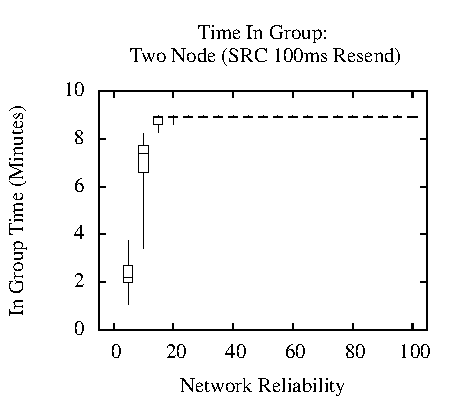
\includegraphics[width=\textwidth]{2NODE-SRC-100-GROUP.pdf}
    \caption{Time in-group over a 10 minute run for a two node system with a 100ms resend time}
    \label{fig:IGT-SRC-2NODE-100}
\end{minipage}%
\qquad
\begin{minipage}{0.45\textwidth}
    \centering
    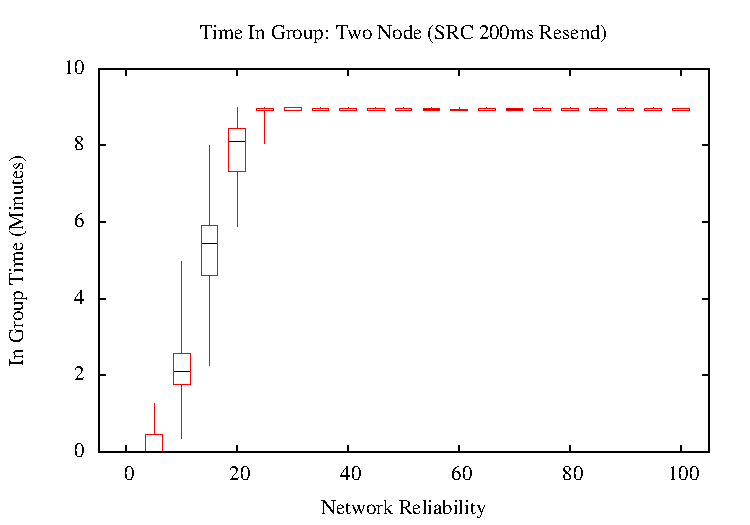
\includegraphics[width=\textwidth]{2NODE-SRC-200-GROUP.pdf}
    \caption{Time in-group over a 10 minute run for a two node system with a 200ms resend time}
    \label{fig:IGT-SRC-2NODE-200}
\end{minipage}
\end{figure}

The 100ms resend SRC test with two nodes can be considered a type of control in this study.
These tests, pictured in Figure \ref{fig:IGT-SRC-2NODE-100}, highlight the performance of the SRC protocol.
The maximum in group time of 9 minutes was achieved with only 15\% of datagrams arriving at the receiver. 

Figure \ref{fig:IGT-SRC-2NODE-200} demonstrates that as the rate at which lost datagrams were re-sent was decreased to 200ms, the in-group time decreased.
This behavior was expected.
Each exchange had a time limit for each message to arrive and the number of attempts was reduced by increasing the resend time.

\subsubsection{Transient Partition Case}

\begin{figure}
\centering
\begin{minipage}{0.45\textwidth}
    \centering
    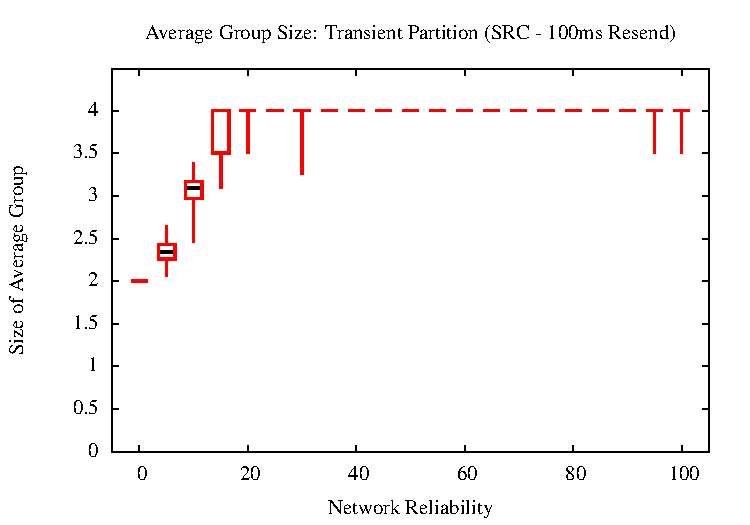
\includegraphics[width=\textwidth]{TRANS-SRC-100-SIZE.pdf}
    \caption{Average size of formed groups for the transient partition case with a 100ms resend time}
    \label{fig:MGS-SRC-TRANS-100}
\end{minipage}%
\qquad
\begin{minipage}{0.45\textwidth}
    \centering
    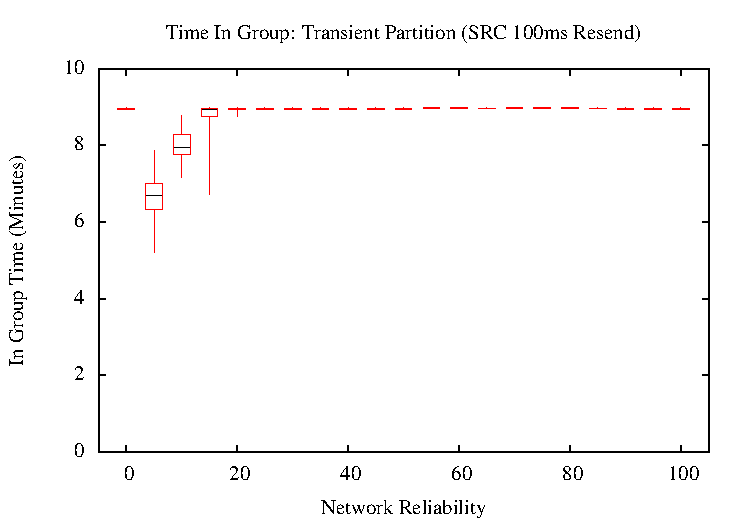
\includegraphics[width=\textwidth]{TRANS-SRC-100-GROUP.pdf}
    \caption{Time in-group over a 10 minute run for the transient partition case with a 100ms resend time}
    \label{fig:IGT-SRC-TRANS-100}
\end{minipage}
\end{figure}

The transient partition case is a simple example in which a network partition separates two groups of DGI processes. In the simplest case where the opposite side of the partition is unreachable, nodes will form a group with the other nodes on the same side of the partition.
In this study, two processes were present on each side of the partition.
In the experiment, the probability of a datagram crossing the partition was increased as the experiment continued.
The 100ms case is shown in Figures \ref{fig:MGS-SRC-TRANS-100} and \ref{fig:IGT-SRC-TRANS-100}.

While messages cannot cross the partition, the DGIs stay in a group with the nodes on the same side of the partition, leading to an in-group time of 9 minutes (the maximum value possible).
As packets began to cross the partition (as the reliability increases), DGI instances on either side attempted to complete elections with the nodes on the opposite partition and the in group time began to decrease.
During this time, however, the mean group size continued to increase.
Thus, while the elections were decreasing the amount of time that the module spent in a state where it can actively do work, it typically did not fall into a state where it was in a group by itself. 
As result, most of the lost in group time comes from elections.

\begin{figure}
\centering
\begin{minipage}{0.45\textwidth}
    \centering
    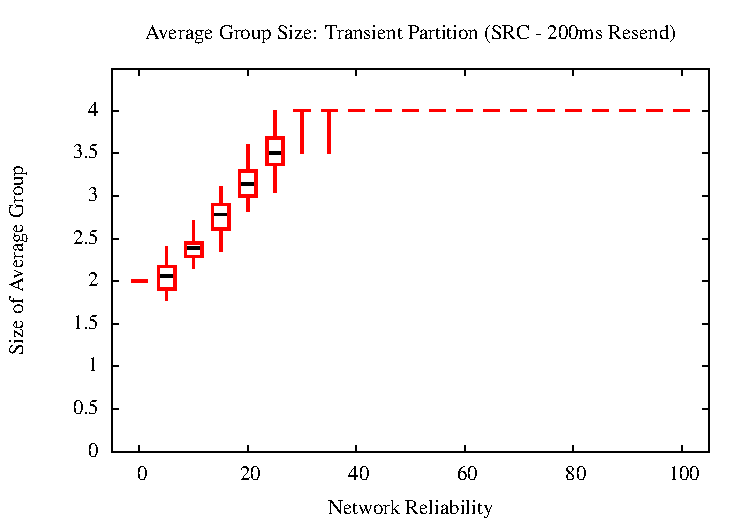
\includegraphics[width=\textwidth]{TRANS-SRC-200-SIZE.pdf}
    \caption{Average size of formed groups for the transient partition case with a 200ms resend time}
    \label{fig:MGS-SRC-TRANS-200}
\end{minipage}%
\qquad
\begin{minipage}{0.45\textwidth}
    \centering
    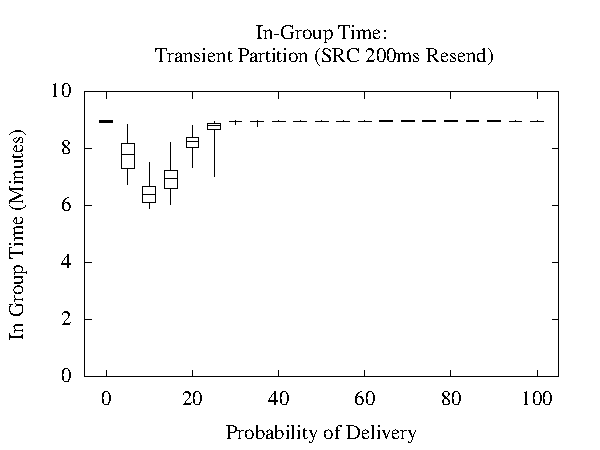
\includegraphics[width=\textwidth]{TRANS-SRC-200-GROUP.pdf}
    \caption{Time in-group over a 10 minute run for the transient partition case with a 200ms resend time}
    \label{fig:IGT-SRC-TRANS-200}
\end{minipage}
\end{figure}

The 200ms case (Illustrated in Figures \ref{fig:MGS-SRC-TRANS-200} and \ref{fig:IGT-SRC-TRANS-200}) suggests a similar behavior to Figures \ref{fig:MGS-SRC-TRANS-100} and \ref{fig:IGT-SRC-TRANS-100}, with a wider valley produced by the reduced number of datagrams.
The mean group size dips below 2 in Figure \ref{fig:MGS-SRC-TRANS-200}, possibly because longer resend times allowed for a greater number race conditions between potential leaders.
Discussion of these race conditions is shown and discussed during the SUC section since it was more prevalent in those experiments.

\subsection{Sequenced Unreliable Connection}

\subsubsection{Two Node Case}

The SUC protocol's experimental tests revealed an immediate problem.
There is a general increasing trend for the amount of time in-group shown in Figure \ref{fig:IGT-SUC-2NODE-100}.
There is a high amount of variance, however, for any particular trial.

\begin{figure}
\centering
\begin{minipage}{0.45\textwidth}
    \centering
    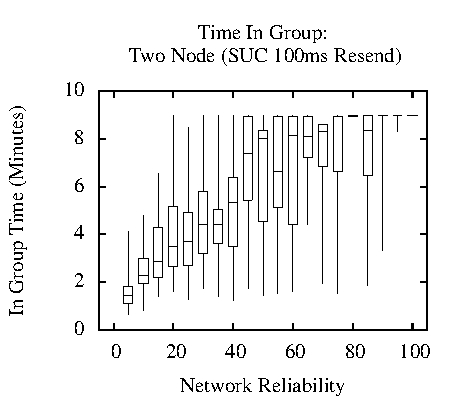
\includegraphics[width=\textwidth]{2NODE-SUC-100-GROUP.pdf}
    \caption{Time in group over a 10 minute run for two node system with 100ms resend time}
    \label{fig:IGT-SUC-2NODE-100}
\end{minipage}%
\qquad
\begin{minipage}{0.45\textwidth}
    \centering
    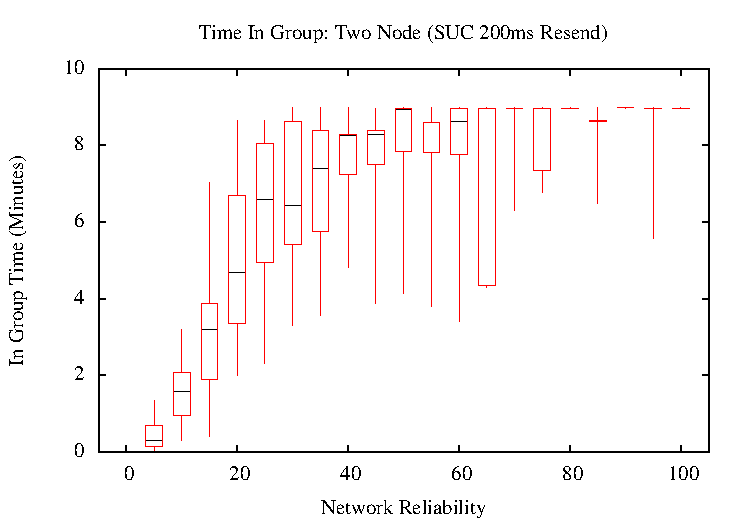
\includegraphics[width=\textwidth]{2NODE-SUC-200-GROUP.pdf}
    \caption{Time in group over a 10 minute run for two node system with 200ms resend time}
    \label{fig:IGT-SUC-2NODE-200}
\end{minipage}
\end{figure}

In the 200ms resend case (illustrated in Figure \ref{fig:IGT-SUC-2NODE-200}), a greater growth rate occurred in the in group time as the reliability increased.
When an average was taken across all of the collected data points from the experiment, the average in group time is higher for the 200ms case than it was for the 100ms case (6.86 vs 6.09).
There large amount of variance in the collected in group time, however.
As a result, it is not possible to state with confidence that the there is a significant difference between the two cases.

\section{Markov Models}

There was high amount of variance in the collected data.
As a result it was difficult to make any sort of prediction about other configurations from the data.
Markov chains were employed to model the system.

\subsection{Initial Model Calibration}

The presented methodology of constructing the model was initially calibrated against the original two-node case.
This calibration used a non-real-time version of the DGI codebase.
The resulting Markov chain was processed using SharpE \cite{SHARPE}\cite{SHARPE2} made by Dr. Kishor Trivedi's group at Duke University, a popular tool for reliability analysis.
SharpE measured the reward collected in 600 seconds, minus the reward that was collected in the first 60 seconds. 
Discarding the reward from the first 60 seconds emulated the 60 seconds were discarded in the experimental runs.
The SharpE results are plotted along with the experimental results in Figures \ref{fig:COMPARE-SUC-2NODE-100} and \ref{fig:COMPARE-SUC-2NODE-200}.

\begin{figure}
\centering
\begin{minipage}{0.45\textwidth}
    \centering
    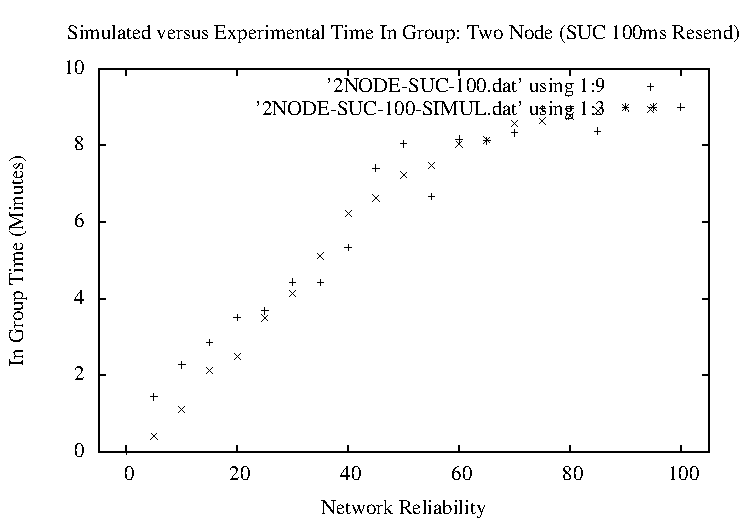
\includegraphics[width=1.0\textwidth]{2NODE-SUC-100-COMPARE.pdf}
    \caption{Comparison of in-group time as collected from the experimental platform and the simulator (1 tick offset between processes).}
    \label{fig:COMPARE-SUC-2NODE-100}
\end{minipage}%
\qquad
\begin{minipage}{0.45\textwidth}
    \centering
    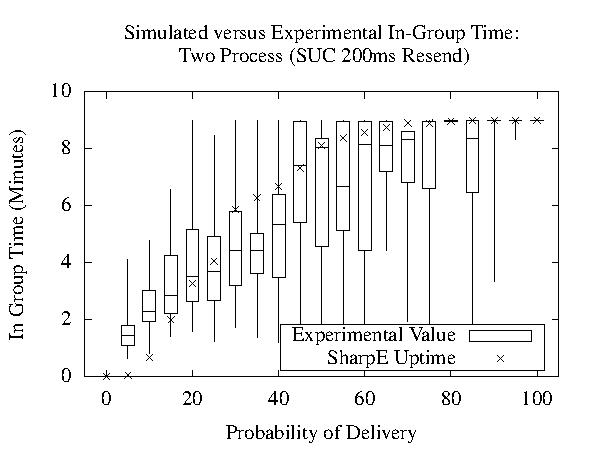
\includegraphics[width=1.0\textwidth]{2NODE-SUC-200-COMPARE.pdf}
    \caption{Comparison of in-group time as collected from the experimental platform and the simulator (2 tick offset between processes).}
    \label{fig:COMPARE-SUC-2NODE-200}
\end{minipage}
\end{figure}

The race condition between processes during an election is a consideration in the original leader election algorithm, and is an additional factor here.
The simulator provided a parameter to allow the operator to select how closely synchronized the peers were.
This synchronization was the time difference between when each of them would search for leaders.
The exchange of messages, particularly during an election, had a tendency to synchronize nodes during elections.
Nodes could synchronize even if they did not initially begin in a synchronized state. 
The simulation results aligned best for the 100ms resend case with 1 tick (Approximately 100ms difference in synchronization between processes) and 2 ticks (Approximately 400ms) in the 200ms resend case.

Models fit to the non-real-time code in groups larger than two processes had a poor fit.
This is presumed to be a combination of several factors.
The major source of fault included the structure of the chain. 
Construction of the chain assumes that all processes enter the election state a roughly the same time. 
This was not typically true for more than two processes.
Additionally, the simulator could only assume that the synchronization between processes was fixed.
The coincidental synchronization that occurred in the two node case was suppressed by the increased number of peers.
Furthermore, an issue with SharpE was discovered that prevented the particular structure of the chains produced from being handled correctly.
The election states with only one outbound transition uncovered a bug in the SharpE software.
To circumvent that, issue, SharpE was replaced by a random-walker which generates exponentially distributed numbers and follows the paths of the chain.
Time in group data for models which SharpE cannot process were collected across several hundred trials.

\begin{figure}
\centering
\begin{minipage}{0.45\textwidth}
    \centering
    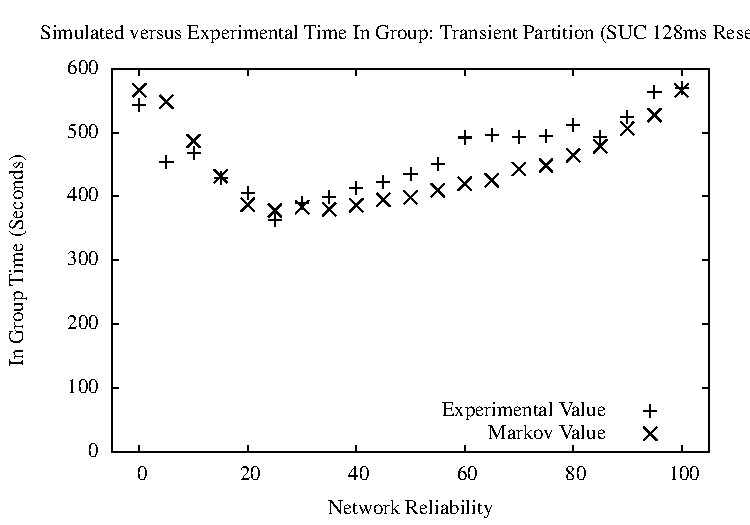
\includegraphics[width=1.0\textwidth]{TRANS-RT-SUC-128-COMPARE.pdf}
    \caption{Comparison of in-group time as collected from the experimental platform and the time in group from the equivalent Markov chain (128ms between resends).}
    \label{fig:COMPARE-SUC-TRANS-RT-128}
\end{minipage}%
\qquad
\begin{minipage}{0.45\textwidth}
    \centering
    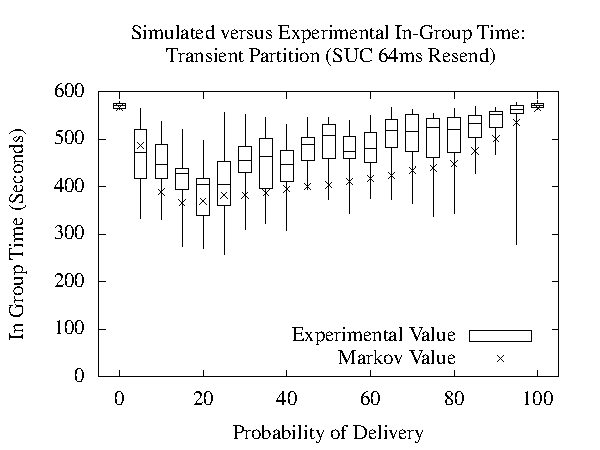
\includegraphics[width=1.0\textwidth]{TRANS-RT-SUC-64-COMPARE.pdf}
    \caption{Comparison of in-group time as collected from the experimental platform and the time in group from the equivalent Markov chain (64ms between resends).}
    \label{fig:COMPARE-SUC-TRANS-RT-64}
\end{minipage}
\end{figure}

The structure of the Markov Chain assumed that processes enter the election state simultaneously.
This was an appropriate assumption for the real-time system, since the round-robin scheduler synchronized when processes ran their group management modules.
The simulator was set to assume that the synchronization between processes was very tight.
New experimental data was collected for the 4 node, transient partition case.
The collected data is overlaid with the results from the random walker in Figures \ref{fig:COMPARE-SUC-TRANS-RT-128} and \ref{fig:COMPARE-SUC-TRANS-RT-64}.

\begin{table}
% increase table row spacing, adjust to taste
\caption{Error and correlation of experimental data and Markov chain predictions}
\label{tab:STAT-DATA}
\centering
% Some packages, such as MDW tools, offer better commands for making tables
% than the plain LaTeX2e tabular which is used here.
\begin{tabular}{|c||c|c|c|}
\hline
Re-send & Correlation & Error \\ \hline
128 & 0.7656 & 11.61\% \\ \hline
64 & 0.8604 & 11.70\% \\ \hline
\end{tabular}
\end{table}

As a measure of the strength of the model, the correlation between the predicted value was compared.
The average error was also computed for each of the samples taken.
This information is presented in Table \ref{tab:STAT-DATA}.
